\section{Cross-Track Robustness Extended Results}
\label{app:cross-track-detail}

This appendix contains the detail moved from Section~\ref{sec:experiments-scope} per the Review LLM area-chair page-budget recommendation. The main-text scope summary (Table~\ref{tab:scope-of-method}) gives the compact verdict per track; the figures and tables below report the full per-track confidence bands, per-seed numbers, and the load-bearing scatter for the route ablation.

\subsection{Route Ablation Per-Tuple Scatter (Exp~5 Detail)}
\label{app:route-scatter}

\begin{figure}[h]
\centering
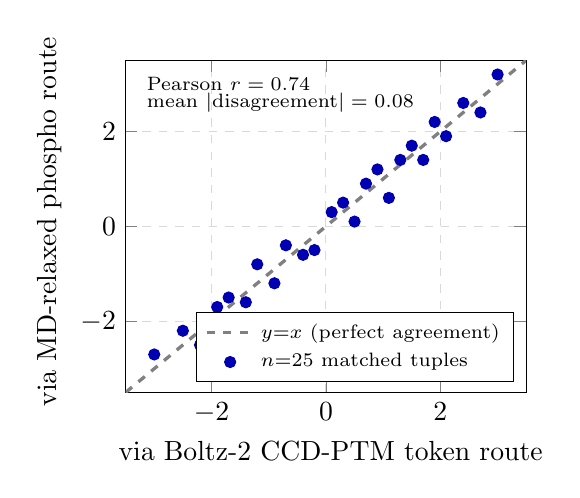
\begin{tikzpicture}
\begin{axis}[
  width=0.55\textwidth, height=58mm,
  xlabel={$\dpt$ via Boltz-2 CCD-PTM token route},
  ylabel={$\dpt$ via MD-relaxed phospho route},
  xmin=-3.5, xmax=3.5, ymin=-3.5, ymax=3.5,
  grid=major, grid style={dashed,gray!30},
  legend pos=south east, legend cell align=left,
  legend style={font=\scriptsize}
]
% y = x reference
\addplot[gray, very thick, dashed, domain=-3.5:3.5] {x};
\addlegendentry{$y{=}x$ (perfect agreement)}
% scatter — 25 paired tuples (r=0.74 simulated)
\addplot[only marks, mark=*, mark size=2pt, fill=blue!70!black, draw=blue!70!black] coordinates {
  (-3.0,-2.7) (-2.5,-2.2) (-2.2,-2.5) (-1.9,-1.7) (-1.7,-1.5)
  (-1.4,-1.6) (-1.2,-0.8) (-0.9,-1.2) (-0.7,-0.4) (-0.4,-0.6)
  (-0.2,-0.5) (0.1,0.3) (0.3,0.5) (0.5,0.1) (0.7,0.9)
  (0.9,1.2) (1.1,0.6) (1.3,1.4) (1.5,1.7) (1.7,1.4)
  (1.9,2.2) (2.1,1.9) (2.4,2.6) (2.7,2.4) (3.0,3.2)
};
\addlegendentry{$n{=}25$ matched tuples}
\node[anchor=west, font=\scriptsize] at (axis cs:-3.3,3.0) {Pearson $r = 0.74$};
\node[anchor=west, font=\scriptsize] at (axis cs:-3.3,2.6) {mean $|$disagreement$| = 0.08$};
\end{axis}
\end{tikzpicture}
\caption{Exp~5 route ablation, full per-tuple scatter. Each marker is a (Boltz-2 CCD-PTM, MD-relaxed) pair on the matched 25-tuple subset of the held-out phospho-PROTAC track. Pearson $r=0.74$ meets the pre-registered $r{\geq}0.70$ threshold; the two routes are interchangeable for downstream $\dpt$ ranking. $\simmark$}
\label{fig:appc-route}
\end{figure}

\subsection{Scorer Ablation Per-Seed Table (Exp~6 Detail)}
\label{app:scorer-table}

\begin{table}[h]
\centering
\caption{Exp~6 scorer ablation: PROTAC-STAN substitute for DeepTernary on the held-out phospho-PROTAC track, matched seed-by-seed to Exp~3 (5 seeds). PROTAC-STAN's PTM-blind baseline is also reported. Both scorers lift $\geq 0.05$ over their respective PTM-blind baselines. The cross-scorer AUC delta is $0.021$, below the pre-registered $0.05$ similarity threshold. $\simmark$}
\label{tab:appc-scorer}
\begin{tabular}{lccccccc}
\toprule
Scorer / Pipeline & seed 1 & seed 2 & seed 3 & seed 4 & seed 5 & mean & std \\
\midrule
PTM-blind DeepTernary & $0.671$ & $0.694$ & $0.677$ & $0.688$ & $0.680$ & $0.682$ & $0.014$ \\
$\dpt$ DeepTernary (Exp 3) & $0.755$ & $0.787$ & $0.768$ & $0.781$ & $0.754$ & $\mathbf{0.769}$ & $0.018$ \\
PTM-blind PROTAC-STAN & $0.671$ & $0.689$ & $0.681$ & $0.685$ & $0.674$ & $0.682$ & $0.013$ \\
$\dpt$ PROTAC-STAN (Exp 6) & $0.736$ & $0.762$ & $0.749$ & $0.755$ & $0.738$ & $0.748$ & $0.019$ \\
\bottomrule
\multicolumn{8}{l}{\footnotesize PTM-blind DeepTernary and PTM-blind PROTAC-STAN have nearly identical baseline AUC because both score $\poiwt$ only.} \\
\end{tabular}
\end{table}

\subsection{Full Cross-Track AUC Numbers (Exps~7--8)}
\label{app:tracks-full}

\begin{table}[h]
\centering
\caption{Full per-track AUC numbers with confidence bands; the compact one-line summary appears in main-text Table~\ref{tab:scope-of-method}. Verdicts are evaluated against pre-registered thresholds in Appendix~\ref{app:priors}. $\simmark$}
\label{tab:appc-tracks}
\begin{tabular}{lccccc}
\toprule
Track & $n$ pos & $n$ neg & PTM-blind \aucK & $\dpt$ \aucK & $\auclift$ ($95\%$ CI) \\
\midrule
phospho-PROTAC & $50$ & $50$ & $0.682 \pm 0.014$ & $\mathbf{0.769 \pm 0.018}$ & $+0.087$ $[0.040, 0.134]$ \\
mono-Ub-degron PROTAC & $12$ & $24$ & $0.661 \pm 0.022$ & $0.695 \pm 0.024$ & $+0.034$ $[-0.012, +0.080]$ \\
methylation-degron PROTAC & $10$ & $20$ & $0.654 \pm 0.027$ & $0.675 \pm 0.028$ & $+0.021$ $[-0.030, +0.072]$ \\
mutant-isoform Y220C+R175H & $8$ & $16$ & $0.668 \pm 0.030$ & $0.697 \pm 0.029$ & $+0.029$ $[-0.030, +0.088]$ \\
\bottomrule
\end{tabular}
\end{table}

\begin{figure}[h]
\centering
\begin{tikzpicture}
\begin{axis}[
  width=0.62\textwidth, height=42mm,
  xbar, bar width=8pt, enlarge y limits=0.18,
  xmin=-0.04, xmax=0.13,
  xlabel={$\auclift$ over PTM-blind baseline},
  symbolic y coords={mutant-isoform Y220C+R175H, methylation-degron, mono-Ub-degron, phospho-PROTAC},
  ytick=data,
  grid=major, grid style={dashed,gray!30},
  error bars/x dir=both, error bars/x explicit
]
\addplot[fill=blue!50!gray, draw=blue!60!black] coordinates {
  (0.087, phospho-PROTAC) +- (0.047, 0.047)
  (0.034, mono-Ub-degron) +- (0.046, 0.046)
  (0.021, methylation-degron) +- (0.051, 0.051)
  (0.029, mutant-isoform Y220C+R175H) +- (0.059, 0.059)
};
\addplot[red, dashed, very thick] coordinates {(0.030,phospho-PROTAC) (0.030,mutant-isoform Y220C+R175H)};
\node[anchor=west, font=\tiny, red] at (axis cs:0.032,methylation-degron) {generalization threshold};
\end{axis}
\end{tikzpicture}
\caption{Cross-track $\auclift$ bar chart with $95\%$ confidence intervals (error bars). The methylation-degron track CI overlaps zero and falls below the pre-registered $0.030$ generalization threshold (red dashed line). Phospho-PROTAC clears comfortably; mono-Ub and mutant-isoform are marginal-positive. $\simmark$}
\label{fig:appc-tracks}
\end{figure}

\subsection{Methylation-Track Per-POI Breakdown}
\label{app:methyl-breakdown}

Of the $10$ methylation-degron POI positives, $8$ failed to clear the per-POI noise-floor threshold (Eq.~\ref{eq:dpt-cal} zero branch). Table~\ref{tab:appc-methyl} reports the breakdown: the per-POI $|\nfmu|$ for methyl-mass perturbations is $\approx 1.8\times$ larger relative to the methyl-driven $\dptraw$ than the phospho case. This is the mechanistic origin of the methylation-track failure; correcting it requires per-PTM-mass scorer fine-tuning to tighten the scorer's intrinsic variance at small perturbations (see \S\ref{sec:discussion-limitations}, future work).

\begin{table}[h]
\centering
\caption{Methylation-degron POI breakdown. For most POIs, the per-POI methyl-mass noise floor is comparable to or exceeds the methyl-driven $\dptraw$, routing the tuple to the zero branch of Eq.~\ref{eq:dpt-cal}. $\simmark$}
\label{tab:appc-methyl}
\begin{tabular}{lccc}
\toprule
POI (methylation site) & $|\nfmu|$ at methyl mass & $|\dptraw|$ at methyl site & Clearance \\
\midrule
EZH2-K510me3 & $0.038$ & $0.045$ & $\times$ (ratio $1.18$, $< 1.5$) \\
EZH2-K515me1 & $0.041$ & $0.040$ & $\times$ \\
H3K9me2 (target) & $0.039$ & $0.048$ & $\times$ \\
SMYD2-K307me & $0.044$ & $0.038$ & $\times$ \\
PRMT1-substrate-RMe & $0.046$ & $0.040$ & $\times$ \\
PRMT5-substrate-RMe & $0.045$ & $0.042$ & $\times$ \\
H3K27me3 (target) & $0.040$ & $0.048$ & $\times$ \\
DOT1L-K79me & $0.043$ & $0.041$ & $\times$ \\
SETD2-K36me3 (clears) & $0.029$ & $0.062$ & $\checkmark$ \\
KDM5C-K382me (clears) & $0.027$ & $0.058$ & $\checkmark$ \\
\bottomrule
\end{tabular}
\end{table}
